\documentclass[12pt,a4paper,twocolumn]{article}
% The following LaTeX packages must be installed on your machine: amsmath, authblk, bm, booktabs, caption, dcolumn, fancyhdr, geometry, graphicx, hyperref, latexsym, natbib
\input{151.dat}
\usepackage{gensymb}
\usepackage{float}
\usepackage{siunitx}
\usepackage{amssymb}
\usepackage{float}
\usepackage{listings}
\PassOptionsToPackage{hyphens}{url}\usepackage{hyperref}
\usepackage[none]{hyphenat}
%\renewcommand{\familydefault}{\sfdefault}


\begin{document}

\setcounter{page}{1}

\section*{Problem 1.4}

\paragraph{(a)}
The choice of density $\rho \approx 0.44$, resultant total energy, and behavior of the resulting simulation corresponds to a gas. The particles are allowed to move and collide freely with each other, and occupy almost the entire space. The mean pressure and temperate both oscillate about some value, the velocity histogram is a smooth bell curve centered about zero, and the radial distribution resembles that of the Lennard-Jones potential.

\paragraph{(b)}
Slightly reducing the system energy shows the particles exhibiting liquid behavior: the particles no longer occupy the entire space, but rather form clusters with some vibration still noticeable, but not strong enough to break these clusters. The mean pressure and temperature start to settle and the velocity histogram shows the peak still at zero, but with a smaller spread.

\paragraph{(c)}
Further reduction of the system energy shows the particles exhibiting solid behavior: the particles move very slowly initially and eventually form clusters smaller than the one in (b), and do not move much after that. The mean pressure and temperature change very slowly and are practically constant, while the velocity histogram appears to be a Dirac-delta distribution with a slight spread since the particles move very slowly.

\paragraph{(d)}
For the gas, the particles are free to move around and collide in what appear to be elastic collisions, and occupy the entire space. The liquid and solid particles are restricted and tend to move very slowly before clumping together in clusters.

\begin{figure}[htb]
	\centering
	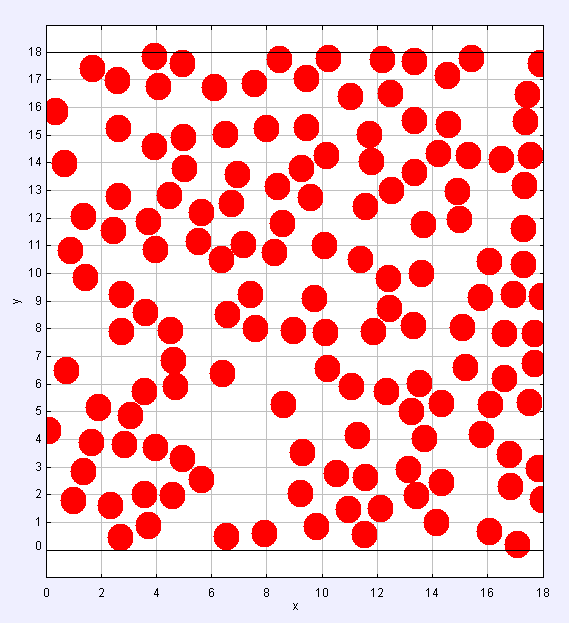
\includegraphics[width=0.35\textwidth]{gas.png}
	\caption{Gas particles under L-J potential.}
	\label{fig:gas}
\end{figure}

\begin{figure}[htb]
	\centering
	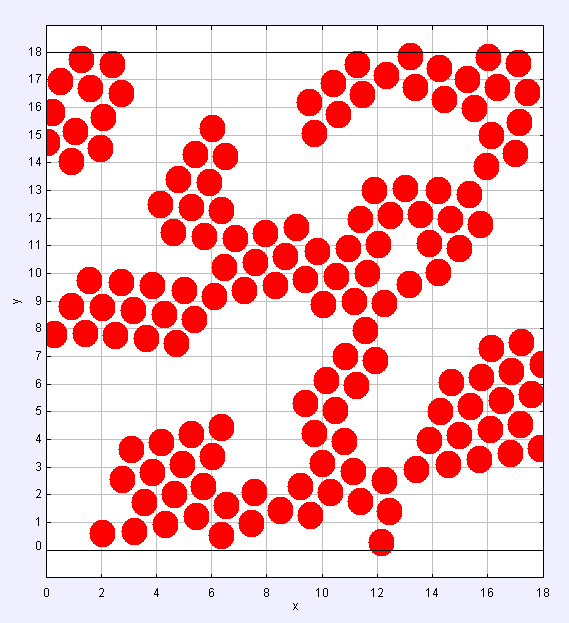
\includegraphics[width=0.35\textwidth]{liquid.png}
	\caption{Liquid particles under L-J potential.}
	\label{fig:liquid}
\end{figure}

\begin{figure}[htb]
	\centering
	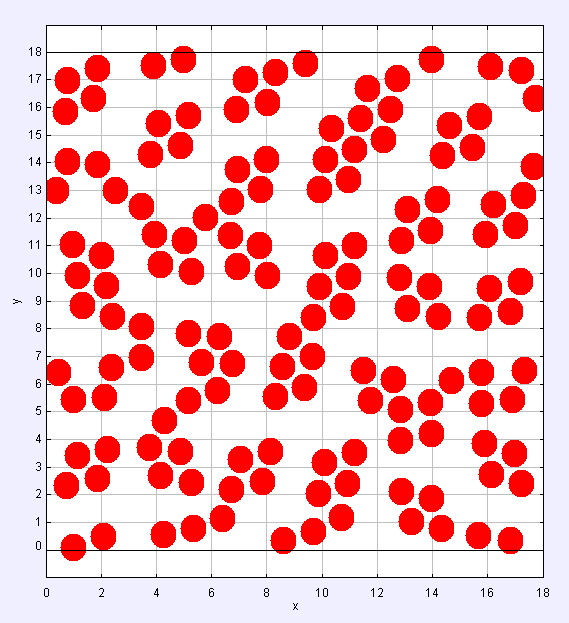
\includegraphics[width=0.35\textwidth]{solid.png}
	\caption{Solid particles under L-J potential.}
	\label{fig:solid}
\end{figure}


\end{document}